\section{Littérature, contexte scientifique et objectifs du projet}
\label{sec:etats_de_art}

Ce section présente le contexte scientifique dans lequel s'inscrivent les travaux réalisés durant ce projet. \\

Il introduit les principaux concepts nécessaires à la compréhension des développements présentés dans les sections suivantes. Nous présenterons tout d'abord les principes de l'ingénierie dirigée par les modèles ainsi que le fonctionnement général d'une chaîne de compilation. Nous introduirons ensuite les notions de théorie du contrôle mobilisées durant ce projet avant de présenter les principales problématiques auxquelles répondent les développements réalisés. \\

\subsection{Contexte scientifique}

Les systèmes embarqués et les systèmes cyber-physiques occupent aujourd'hui une place importante dans de nombreux domaines industriels tels que la robotique, les transports, l'aéronautique ou encore les systèmes autonomes. Ces systèmes combinent des composants logiciels, des dispositifs matériels, des capteurs et des actionneurs devant interagir de manière fiable dans des environnements souvent complexes et évolutifs. Leur conception représente un défi important, tant par le nombre de composants impliqués que par les nombreuses interactions existant entre eux. \\

Afin de maîtriser cette complexité, l'ingénierie dirigée par les modèles (Model-Driven Engineering, MDE) propose de placer les modèles au coeur du processus de développement. Plutôt que de développer directement une application sous forme de code source, les systèmes sont d'abord décrits à un niveau d'abstraction élevé au moyen de modèles. Ces derniers peuvent ensuite être analysés, transformés et progressivement raffinés jusqu'à produire du code exécutable. Cette approche améliore la maintenabilité des systèmes, facilite leur évolution et permet d'automatiser une partie importante du développement logiciel grâce aux transformations de modèles. \\

Dans cette approche, les langages spécifiques à un domaine (Domain-Specific Languages, DSL) occupent une place centrale. Contrairement aux langages généralistes, ils offrent des abstractions directement adaptées à un domaine d'application particulier, permettant aux concepteurs d'exprimer plus naturellement les concepts manipulés tout en réduisant les risques d'erreurs. Le langage CHIPS s'inscrit dans cette philosophie. Développé dans le cadre du projet ANR ADAPT, il est destiné à la modélisation de systèmes distribués hiérarchiques et sa compilation repose sur les principes du langage BIP (Behavior, Interaction, Priority), largement utilisé pour la modélisation formelle de systèmes à composants hétérogènes \cite{basu2011bip}. CHIPS permet ainsi de décrire des systèmes complexes tout en conservant une représentation exploitable par des outils de simulation, de vérification formelle et de génération de code. \\

Une chaîne de compilation destinée à un tel langage repose sur plusieurs étapes complémentaires. Dans un premier temps, le programme est soumis à une analyse lexicale, qui consiste à transformer la suite de caractères du fichier source en une suite de termes. Cette étape est suivie d'une analyse syntaxique, dont l'objectif est de vérifier que ces lexèmes respectent la grammaire du langage et de construire un arbre syntaxique abstrait (AST). L'AST constitue une représentation structurée du programme indépendante de sa syntaxe textuelle. \\

Une fois cet arbre obtenu, une analyse sémantique est réalisée. Celle-ci dépasse largement la simple vérification grammaticale puisqu'elle consiste notamment à contrôler le typage, la cohérence des déclarations, la visibilité des identifiants ou encore les règles de portée des variables. Ces vérifications nécessitent généralement l'utilisation d'une table des symboles, structure fondamentale dans la conception des compilateurs, permettant d'associer à chaque identifiant l'ensemble des informations nécessaires à son interprétation. \\

Dans le cadre de CHIPS, cette analyse sémantique est suivie d'une phase de génération de modèles XMI conforme au méta-modèle Ecore utilisé par l'Eclipse Modeling Framework (EMF). Cette représentation intermédiaire permet ensuite aux différents outils de la chaîne de compilation de manipuler le programme sous une forme standardisée avant sa transformation vers les représentations utilisées par le compilateur BIP. L'organisation générale de cette chaîne est présentée sur la figure \ref{fig:architecture_modif}. \\

Les premières versions du compilateur CHIPS reposaient sur les outils Flex, Bison et Yacc, particulièrement répandus dans le développement de compilateurs. Cette architecture a permis de démontrer la faisabilité du projet et de produire une partie de la chaîne de compilation fonctionnelle, qui est celle du parseur. Cependant, l'évolution progressive du langage a rapidement fait apparaître plusieurs limitations. L'introduction des templates C++, utilisées pour représenter les classes lors de la création de l'AST, rend notamment cette création plus complexe car les templates ne sont pas directement supportés par Bison. Afin de faciliter l'évolution du langage, une migration vers ANTLR4 a été envisagée. Cet outil permet de produire une grammaire plus lisible, plus modulaire et généralement plus simple à maintenir que Bison. De plus, ANTLR4 permet l'utilisation de templates C++ dans les actions de la grammaire, ce qui simplifie la création de l'AST. \\


Au-delà des évolutions du compilateur, CHIPS vise également à intégrer directement dans le langage des mécanismes issus de la théorie du contrôle. Les systèmes cyber-physiques reposent en effet sur des boucles d'asservissement utilisant les mesures fournies par des capteurs afin de commander des actionneurs. La qualité de ces mesures conditionne directement les performances du système de commande. \\

Parmi les régulateurs existants, le contrôleur PID (Proportional-Integral-Derivative) demeure aujourd'hui le plus largement utilisé dans l'industrie. De nombreuses études estiment que plus de 90 \% des boucles de régulation industrielles utilisent encore un régulateur de type PI ou PID en raison de leur simplicité de mise en oeuvre, de leur faible coût de calcul et de leur robustesse pour un très grand nombre de procédés industriels \cite{aastrom2006}.
Son principe consiste à combiner trois actions complémentaires : une action proportionnelle corrigeant instantanément l'erreur, une action intégrale supprimant les erreurs permanentes et une action dérivée permettant d'anticiper les variations du système. Malgré l'apparition de méthodes de commande plus avancées telles que la commande optimale ou la commande prédictive, les PID restent aujourd'hui la solution privilégiée dans de nombreux systèmes industriels grâce à leur excellent compromis entre simplicité et performances. \\

L'utilisation d'un PID soulève néanmoins deux difficultés majeures rencontrées dans la plupart des applications réelles. \\

La première concerne les mesures issues des capteurs. Les capteurs sont soumis à différentes perturbations : bruit électronique, vibrations mécaniques, erreurs de mesure, perturbations environnementales ou encore quantification numérique. Si ces perturbations sont directement utilisées par le contrôleur, elles peuvent provoquer des oscillations de la commande, une diminution de la stabilité ou une dégradation des performances du système. Il est donc nécessaire d'effectuer un prétraitement des signaux avant leur exploitation. \\

Les filtres numériques constituent l'une des solutions les plus utilisées pour répondre à cette problématique. Les filtres passe-bas permettent d'atténuer les composantes de haute fréquence tout en conservant les variations lentes correspondant généralement au signal utile. 
A l'inverse, les filtres passe-haut suppriment dans un signal les composantes de basse fréquence. Parmi les nombreuses familles de filtres existantes, les filtres de Butterworth, proposés par Stephen Butterworth en 1930, sont particulièrement utilisés en automatique car ils présentent une réponse fréquentielle maximalement plate dans la base passante, c'est-à-dire sans ondulations, tout en offrant une pente d'atténuation plus importante que les filtres du premier ordre \cite{butterworth1930}. Leur conception ainsi que leurs propriétés sont largement décrites dans les ouvrages de référence consacrés au traitement numérique du signal \cite{oppenheim2010,orfanidis1996}. Ces caractéristiques en font un excellent compromis entre coût de calcul, stabilité numérique et efficacité du filtrage. \\


La seconde difficulté apparaît lorsque la commande calculée par le PID dépasse les capacités physiques de l'actionneur. Dans cette situation, l'actionneur entre en saturation tandis que le terme intégral du PID continue d'accumuler l'erreur. Ce phénomène, connu sous le nom d'integral windup, provoque généralement une augmentation importante du dépassement, un ralentissement du temps de réponse ainsi qu'une perte de stabilité transitoire. Ce problème est particulièrement fréquent dans les systèmes réels où les actionneurs possèdent nécessairement des limites physiques. \\

Afin de limiter ces effets, de nombreuses stratégies d'anti-windup ont été proposées dans la littérature. Les deux approches les plus couramment utilisées sont le clamping, qui consiste à suspendre ou limiter l'intégration lorsque la commande est saturée, et le back-calculation, qui réinjecte l'erreur de saturation dans l'intégrateur afin d'accélérer son retour vers une valeur cohérente. Ces méthodes sont aujourd'hui largement employées dans les applications industrielles car elles permettent d'améliorer significativement le comportement transitoire des régulateurs PID tout en conservant une mise en oeuvre relativement simple. Une synthèse détaillée de ces approches est proposée par Tarbouriech et Turner, qui présentent également les principales problématiques de recherche encore ouvertes dans ce domaine \cite{tarbouriech2009}. \\

\subsection{Objectifs}

Les travaux réalisés durant ce stage s'inscrivent dans cette double problématique. D'une part, ils visent à faire évoluer l'infrastructure du compilateur CHIPS afin d'améliorer sa maintenabilité, son extensibilité et sa capacité à prendre en charge les nouvelles évolutions du langage. D'autre part, ils enrichissent la bibliothèque de composants du langage en intégrant plusieurs outils issus de la théorie du contrôle directement réutilisables dans les modèles CHIPS. \\

Plus précisément, les objectifs de ce stage sont les suivants :
\begin{itemize}
    \item migrer le parseur historique vers ANTLR4 afin d'obtenir une architecture plus robuste et plus 
    facilement extensible
    \item adapter le générateur XMI au nouvel arbre syntaxique produit par ANTLR4
    \item développer une bibliothèque de filtres numériques comprenant des filtres passe-bas, passe-haut, 
    Butterworth d'ordre 2 ainsi qu'un filtre médian
    \item implémenter plusieurs mécanismes d'anti-windup destinés aux contrôleurs PID, notamment les 
    approches Clamp et Back-calculation
    \item intégrer l'ensemble de ces composants à la chaîne de compilation CHIPS
    \item évaluer expérimentalement les performances des différentes solutions proposées au moyen d'analyses 
    temporelles, fréquentielles et de mesures de performances de la chaîne de compilation.
\end{itemize}

L'ensemble de ces travaux contribue ainsi à renforcer la maturité du langage CHIPS aussi bien du point de vue de son infrastructure logicielle que des fonctionnalités pour la modélisation de systèmes cyber-physiques adaptatifs. \\

\begin{figure}
    \centering
    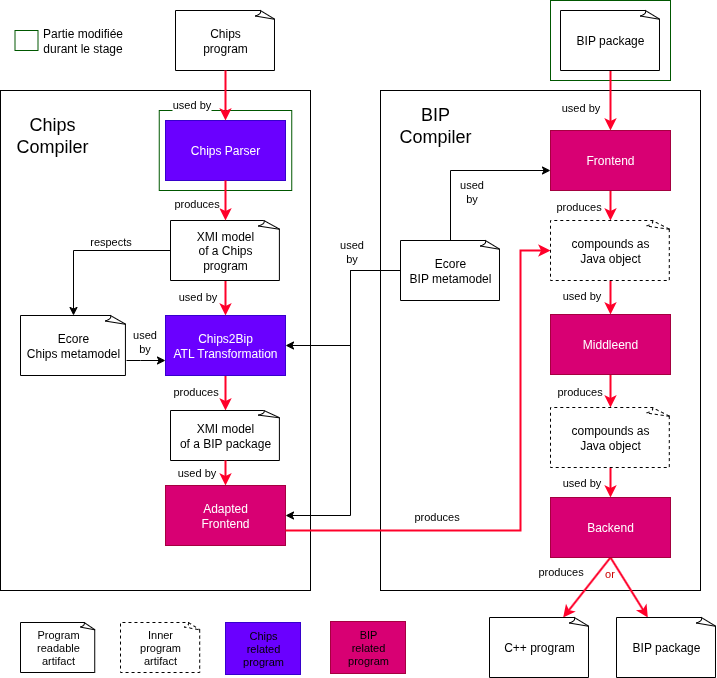
\includegraphics[width=\textwidth]{images/architecture_partie_modifier.png}
    \caption{Architecture de base avec les parties modifiées}
    \label{fig:architecture_modif}
\end{figure}

\FloatBarrier

\newpage%